\documentclass[10pt]{article}
\usepackage{graphicx} % Required for inserting images
\usepackage{url}
\usepackage{hyperref}
\title{IEG_Problems_Lecture1}
\author{martavictoriaperez }
\date{December 2024}

\usepackage[margin=1in]{geometry} 
\usepackage{amsmath,amsthm,amssymb, graphicx, multicol, array}
 
\newcommand{\N}{\mathbb{N}}
\newcommand{\Z}{\mathbb{Z}}
 
\newenvironment{problem}[2][Problem]{\begin{trivlist}
\item[\hskip \labelsep {\bfseries #1}\hskip \labelsep {\bfseries #2.}]}{\end{trivlist}}

\begin{document}
 
\title{\textbf{Lecture 6: Gas networks}}
\author{
%Your name\\
DTU Course 46770: Integrated Energy Grids }
\maketitle

\begin{problem}{6.1}

Consider the simplified network plotted in Fig. \ref{fig_network}, which represents Denmark and its neighbouring countries. Assume that the nodes are connected using transmission methane gas pipelines.


\begin{figure}
    \centering
    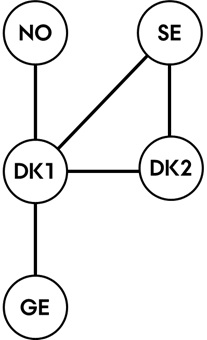
\includegraphics[width=0.2\linewidth]{figures/nodes.jpg}
    \caption{Simplified network.}
    \label{fig_network}
\end{figure}
\begin{itemize}

\item[a)] Calculate the capacity of every pipeline (in MW) assuming that they operate at a pressure $P$=50 bar, the average flow velocity is $u$ = 15 m/s, the diameter of the pipe is $d$ = 600mm and the energy content of methane is 50 GJ/tonne. To calculate the speed of sound in gas $c$, assume the universal gas constant $R$=8.314 J/mol, the molar mass of methane $M$=16 g/mol, compression factor $Z$=1.31, and 25$^{\circ}$C.

\item[b)] Assuming steady-state conditions, use link elements in PyPSA to build a network like the one shown in Fig. 1.  Assume that, in the first time step,  in every node, there is a demand for 5 GWh of methane.  In the Norway node, there is a gas generator with a marginal cost 20 EUR/MWh$_{th}$, in the Sweden node, there is a gas generator with a marginal cost of 10 EUR/$MWh_{th}$, calculate the optimal gas flows through the network and plot them. 

\item[c)] Assume the following lengths for the links: DK1-DK2=200 km, DK1-DE=600 km, DK1-NO= 500 km, DK1-SE=600 km, DK2-SE=100 km. If we consider that the losses due to energy consumption to maintain the pressure can be estimated at 2\% of the energy flow per 1000 km. Adapt the link elements in PyPSA to include an efficiency that takes compression energy demand into account, and calculate the optimal gas flows through the network and plot them.

\item[d)] Assuming the following demands in GWh for three consecutive time steps DK1=[1,2,1], DK2=[1,1,1], DE=[1,2,3], NO=[1,1,1], SE=[0,1,0]. Calculate the optimal flows in every time step and the total system costs. 

\item[e)] Assume that the pipeline pressure can be increased to 25 bar, calculate the linepack, i.e., the energy that can be stored in every pipeline by increasing the pressure. Represent this in your PyPSA model by adding a store with that capacity at the beginning of every line, calculate the optimal gas flows in every time step and the total system costs.

\end{itemize}


\end{problem}

\

\begin{problem}{6.2}
Let us assume that the countries in Problem 6.1 are considering repurposing their methane gas network into a hydrogen network. In order to run the existing pipelines with hydrogen, the pressure needs to be reduced to $P$=40 bar, and the average flow velocity can be increased to $u$ = 30 m/s. Calculate the capacity of every pipeline (in MW), and relative to their initial design when they transport methane gas. 

The energy content of $H_2$ is 120 GJ/tonne. To calculate the speed of sound in hydrogen $c$, assume the universal gas constant $R$=8.314 J/mol, the molar mass of hydrogen $M$=2 g/mol, compression factor $Z$=1.03, and 25$^{\circ}$C.


\end{problem}



%\begin{proof}[Solution]
%Write a solution here
%\end{proof}

\end{document}


 

